

\PassOptionsToPackage{table}{xcolor}
\documentclass[aspectratio=169]{beamer}\usepackage[]{graphicx}\usepackage[]{color}
%% maxwidth is the original width if it is less than linewidth
%% otherwise use linewidth (to make sure the graphics do not exceed the margin)
\makeatletter
\def\maxwidth{ %
  \ifdim\Gin@nat@width>\linewidth
    \linewidth
  \else
    \Gin@nat@width
  \fi
}
\makeatother

\definecolor{fgcolor}{rgb}{0.345, 0.345, 0.345}
\newcommand{\hlnum}[1]{\textcolor[rgb]{0.686,0.059,0.569}{#1}}%
\newcommand{\hlstr}[1]{\textcolor[rgb]{0.192,0.494,0.8}{#1}}%
\newcommand{\hlcom}[1]{\textcolor[rgb]{0.678,0.584,0.686}{\textit{#1}}}%
\newcommand{\hlopt}[1]{\textcolor[rgb]{0,0,0}{#1}}%
\newcommand{\hlstd}[1]{\textcolor[rgb]{0.345,0.345,0.345}{#1}}%
\newcommand{\hlkwa}[1]{\textcolor[rgb]{0.161,0.373,0.58}{\textbf{#1}}}%
\newcommand{\hlkwb}[1]{\textcolor[rgb]{0.69,0.353,0.396}{#1}}%
\newcommand{\hlkwc}[1]{\textcolor[rgb]{0.333,0.667,0.333}{#1}}%
\newcommand{\hlkwd}[1]{\textcolor[rgb]{0.737,0.353,0.396}{\textbf{#1}}}%

\usepackage{framed}
\makeatletter
\newenvironment{kframe}{%
 \def\at@end@of@kframe{}%
 \ifinner\ifhmode%
  \def\at@end@of@kframe{\end{minipage}}%
  \begin{minipage}{\columnwidth}%
 \fi\fi%
 \def\FrameCommand##1{\hskip\@totalleftmargin \hskip-\fboxsep
 \colorbox{shadecolor}{##1}\hskip-\fboxsep
     % There is no \\@totalrightmargin, so:
     \hskip-\linewidth \hskip-\@totalleftmargin \hskip\columnwidth}%
 \MakeFramed {\advance\hsize-\width
   \@totalleftmargin\z@ \linewidth\hsize
   \@setminipage}}%
 {\par\unskip\endMakeFramed%
 \at@end@of@kframe}
\makeatother

\definecolor{shadecolor}{rgb}{.97, .97, .97}
\definecolor{messagecolor}{rgb}{0, 0, 0}
\definecolor{warningcolor}{rgb}{1, 0, 1}
\definecolor{errorcolor}{rgb}{1, 0, 0}
\newenvironment{knitrout}{}{} % an empty environment to be redefined in TeX

\usepackage{alltt}

\mode<presentation>
{
  \usetheme{Warsaw}
  
}

\beamertemplatenavigationsymbolsempty 

\usepackage[]{inputenc}
\usepackage[english]{babel}
\usepackage{amsthm}
\usepackage{graphicx}
\usepackage{epstopdf}
\usepackage{grffile}
\usepackage{hyperref}
\usepackage{beamerthemesplit}
\definecolor{links}{HTML}{2A1B81}
\hypersetup{colorlinks,linkcolor=,urlcolor=links}
%\setsansfont[Ligatures={Common,TeX}]{TeX Gyre Heros}

{\renewcommand{\arraystretch}{1.1}

\AtBeginSection[]
{
  \begin{frame}
    \frametitle{Outline}
    \tableofcontents[currentsection]
  \end{frame}
}

\newcommand*\oldmacro{}%
\let\oldmacro\insertshorttitle%
\renewcommand*\insertshorttitle{%
   \oldmacro\hfill%
   \insertframenumber\,/\,\inserttotalframenumber}

\setbeamertemplate{headline}{}
\setbeamertemplate{itemize items}[circle]
\title{Parallel \textbf{R}}

\author [Andrew Bzikadze]{Andrew Bzikadze\\ \texttt{\small{\href{mailto:seryrzu@gmail.com}{seryrzu@gmail.com}}}}
\institute{Saint Petersburg State University, Russia \\
           Faculty of Mathematics and Mechanics \\
           Department of Statistical Modelling}
\date {
September 12, 2015
}
\IfFileExists{upquote.sty}{\usepackage{upquote}}{}
\begin{document}
\begin{frame}
  \titlepage
\end{frame}


\section{Motivation and introduction}
\begin{frame}
  \frametitle {Motivation}
  \begin{columns}[T]
    \begin{column}{.48\textwidth}
      Why \textbf{R}? The \textbf{R} language has a lot of advantages:
      \begin{itemize}
        \item Open Source.
        \item Cross-Platform.
        \item Free.
        \item Many basic tools.
        \item \textbf{R} extensions.
        \item Arguable fast with \textbf{R}-way style and well-implemented \textbf{R} distribution.
      \end{itemize}
      
      \pause
      
      Why bother then?
    \end{column}
    \pause
    \begin{column}{.48\textwidth}
     There are 2 major limitations:
      \begin{itemize}
        \item Single-threaded: no out-of-box support of multi-thread calculations.
        \item Memory-bound: all data should fit in RAM.
      \end{itemize}
      
      \pause
      
      \textit{Solution:} {\color{blue} {Parallel Execution.}}
      How exactly?
      \begin{itemize}
        \item Single-threaded: multiple CPU's (and cores).
        \item Memory-bound: spread data from one computer (master) to several computers (slaves).
      \end{itemize}
    \end{column}
  \end{columns}
\end{frame}

\begin{frame}
  \frametitle{Basic Terminology}
  The two types of parallelism:
  \begin{itemize}
    \item \textbf{Implicit} --- the OS abstracts parallelism from the user.
    \item \textbf{Explicit} --- user controls details of the process.
  \end{itemize}
  
  \vspace{2mm}
  A \textbf{computer cluster} consists of a set of loosely or tightly connected computers that work together so that, in many respects, 
  they can be viewed as a single system (Wiki).
  
  \vspace{2mm}
  \textbf{Master/slave} is a model of communication where one device or process has unidirectional control over one or more other devices (Wiki).
  
\end{frame}

\begin{frame}
  \frametitle{Overview}
  \begin{columns}[T]
    \begin{column}{.5\textwidth}
      \begin{table}[]
        \begin{tabular}{ll}
          {\large{\textbf{snow}}} & \\
          \textit{Usage:} & 
            \begin{tabular}[c]{@{}l@{}}
              Explicit parallelism by using \\ clusters (works on Linux, \\ Windows, Mac OS X).
            \end{tabular} \\
          \textit{Solves:} & 
            \begin{tabular}{@{}l@{}}
              Single-threaded,  memory-bound.
            \end{tabular} \\
          & \\
          & \\
          \multicolumn{2}{l} 
            {\large{\textbf{multicore [deprecated]}}} \\
            \textit{Usage:} & 
              \begin{tabular}{@{}l@{}}
                Implicit parallelism by using \\ FORK (doesn't work on \\ Windows).
              \end{tabular} \\
          \textit{Solves:} & Single-threaded.
        \end{tabular}
      \end{table}    
    \end{column}
    
    \pause
   
    \begin{column}{.5\textwidth}
      \begin{table}[]
        \begin{tabular}{ll}
          \multicolumn{2}{l} 
            {\large{\textbf{parallel [mainstream]}}} \\
          \textit{Usage:} & 
            \begin{tabular}{@{}l@{}}
              Almost a wrapper of \texttt{snow} and \\ \texttt{multicore}.
            \end{tabular} \\
          \textit{Solves:} & 
            \begin{tabular}{@{}l@{}}
              Single-threaded, memory-bound.
            \end{tabular} \\
          & \\
          & \\ 
          &
          \pause 
          \\
          \multicolumn{2}{l} 
            {\large{\textbf{Hadoop}}} \\
          \multicolumn{2}{l} 
            {\textbf{R} + \texttt{Hadoop, RHIPE, Segue}.} \\
        \end{tabular}
      \end{table}    
    \end{column}
  \end{columns}
\end{frame}

\begin{frame}
  \frametitle{Epigraph}
  \begin{quote}
    ``\ldots R was not built in anticipation of the Big Data revolution.
    
    R was born in 1995. Disk space was expensive, RAM even more so, and this thing called
    The Internet was just getting its legs. Notions of ``large-scale data analysis'' and ``high-performance
    computing'' were reasonably rare. Outside of Wall Street firms and university
    research labs, there just wasn`t that much data to crunch.''
  \end{quote}
  {\hfill --- Q. Ethan McCallum and Stephen Weston ``Parallel \textbf{R}''}
\end{frame}


\begin{frame}{Outline}
  \tableofcontents%[pausesections]
  % You might wish to add the option [pausesections]
\end{frame}
\section{snow}
\begin{frame}[fragile]
    \frametitle{\texttt{snow}: quick look}

    \begin{table}[]
      \rowcolors{1}{gray!25}{white}
      \centering
      \begin{tabular}{rl}
        \textit{General use case:} & main word is {\color{blue} cluster}, provides {\color{blue} explicit} parallelism. \\
        \textit{Examples:} & \begin{tabular}{@{}l@{}}Monte Carlo simulations, bootstrapping, cross validation, \\ensemble machine learning algorithms. \end{tabular} \\
        \textit{Solves:} & Single-threaded, memory-bound. \\
        \textit{Cool features}: & 
          \begin{minipage}{4in}
            \vskip 4pt
            \begin{itemize}
              \item Different transport mechanisms between Master and Slaves: Sockets, MPI (\texttt {rmpi}), NWS (\texttt{nws}), PVM (\texttt{rpvm}).
              \item Good support of RNG (\texttt{rsprng}, \texttt{rlecuyer}).
            \end{itemize}
            \vskip 4pt
          \end{minipage} \\
        \textit{Problems:} & No communication between the workers (slaves). \\
        \pause
        {\color{blue} \textit{Warning:}} & \begin{tabular}{@{}l@{}} \color{blue} The input arguments \textbf{must fit} into memory when calling\\ \color{blue} \texttt{snow} function. 
        It’s up to the user to
        arrange high-performance \\ \color{blue} distributed file systems. \end{tabular}
      \end{tabular}
    \end{table}
\end{frame}

\begin{frame}
    \frametitle{Structure of API}
%     \begin{itemize}
%       \item \textit{Start and stop clusters}: makeCluster, stopCluster;
%       \item \textit{Low-level (cluster-level) functions}: \texttt{cluster*} --- \texttt{clusterApply}, \texttt{clusterApplyLB}, \texttt{clusterEvalQ}, 
%             \textit{clusterCall}, \texttt{clusterSplit}, etc\ldots;
%       \item \textit{High-level functions}: \texttt{par[L,S,A,R,C]apply} --- parallel versions of apply and related functions;
%       \item \textit{(Uniform) RNG}: L`Ecuyer (pack: \texttt{rlecuyer}), SPRNG \textit{[deprecated]} (package: \texttt{rsprng});
%       \item \textit{Timing}: \texttt{snow.time(expr)} -- very useful.
%     \end{itemize}
    \begin{table}[]
      \rowcolors{1}{gray!25}{white}
      \centering
      \begin{tabular}{rl}
        \textit{Start and stop clusters:} & makeCluster, stopCluster. \\
        \textit{Low-level (cluster-level) functions:} & 
          \begin{tabular}{@{}l@{}}
            \texttt{cluster*} --- \texttt{clusterApply}, \texttt{clusterApplyLB},\\ \texttt{clusterEvalQ}, 
            \texttt{clusterCall}, \texttt{clusterSplit}, etc.
          \end{tabular} \\
        \textit{High-level functions:} &
          \begin{tabular}{@{}l@{}}
              \texttt{par[L,S,A,R,C]apply} --- parallel versions of\\ apply and related functions.
          \end{tabular} \\
        \textit{(Uniform) RNG:} &
          \begin{tabular}{@{}l@{}}
              L`Ecuyer (package: \texttt{rlecuyer}), \\ SPRNG \textit{[deprecated]} (package: \texttt{rsprng}).
          \end{tabular} \\
        \textit{Timing}: & \texttt{snow.time(expr)} --- very useful.
      \end{tabular}
    \end{table}
\end{frame}


\begin{frame}[fragile]
    \frametitle{Start and stop clusters}
    
    Basic way:
\begin{knitrout}
\definecolor{shadecolor}{rgb}{1, 1, 1}\color{fgcolor}\begin{kframe}
\begin{alltt}
  \hlstd{cl} \hlkwb{<-} \hlkwd{makeCluster}\hlstd{(}\hlnum{8}\hlstd{,} \hlkwc{type} \hlstd{=} \hlstr{"SOCK"}\hlstd{)} \hlcom{# or you may use }
                                      \hlcom{# makeSOCKcluster(), }
                                      \hlcom{# makePVMcluster(), etc.}
  \hlkwd{stopCluster}\hlstd{(cl)}
\end{alltt}
\end{kframe}
\end{knitrout}

  First parameter is \texttt{spec} --- specification. It is \texttt{ssh}-configurable unless you type \texttt{"localhost"}:
  
  
<<,background="white"
  cl <- makeCluster(c("localhost","localhost"), type = "SOCK")
  stopCluster(cl)
@

{\color{blue} \textit{Warning:} Be aware of computational costs of cluster setup.}
\end{frame}

\begin{frame}{Low-level API}
  All of them are \texttt{cluster*} and designed for computing {\color{blue} \textit{on}} a cluster. Most interesting are as follows.
%   \begin{itemize}
%     \item \texttt{clusterApply(cl, x, fun, ...)} --- jobs are being ``recycled''.
%     \item \texttt{clusterApplyLB(cl, x, fun, ...)} --- Load Balancing version of clusterApply().
%     \item \texttt{clusterCall(cl, fun, ...)} --- calls a function fun with identical arguments ... on each node in the cluster cl and returns a list of the results.
%     \item \texttt{clusterEvalQ(cl, expr)} --- evaluates an expression expr on each node in the cluster cl; implemented using clusterCall();
%     \item \texttt{clusterMap(cl, fun, ..., MoreArgs = NULL, RECYCLE = TRUE)} --- similar to \texttt{mapply}.
%   \end{itemize} 
  \begin{table}[]
    \rowcolors{1}{gray!25}{white}
    \centering
    \begin{tabular}{ll}
      \texttt{clusterApply(cl, x, fun, ...)} & Jjobs are being ``recycled''.\\
      \texttt{clusterApplyLB(cl, x, fun, ...)} & Load Balancing version of clusterApply(). \\
       \texttt{clusterCall(cl, fun, ...)} & 
         \begin{tabular}{@{}l@{}}
           Calls a function fun with identical \\ arguments ... on each node in the cluster cl \\ and returns a list of the results.
         \end{tabular} \\
       \texttt{clusterEvalQ(cl, expr)} & 
         \begin{tabular}{@{}l@{}}
           Evaluates an expression expr on each node\\ in the cluster cl; \\ implemented using clusterCall().
         \end{tabular} \\
       \begin{tabular}{@{}l@{}}
          \texttt{clusterMap(cl, fun, ...,}\\ \quad \texttt{MoreArgs = NULL, RECYCLE = TRUE)}
        \end{tabular}
        & Similar to \texttt{mapply}.
    \end{tabular}
  \end{table}
\end{frame}

\begin{frame}[fragile]{Example, K-means}


  \begin{columns}[T]
    \begin{column}{.48\textwidth}
      Basic one-core way:
\begin{knitrout}\scriptsize
\definecolor{shadecolor}{rgb}{1, 1, 1}\color{fgcolor}\begin{kframe}
\begin{alltt}
\hlkwd{library}\hlstd{(MASS)}
\hlstd{result} \hlkwb{<-} \hlkwd{kmeans}\hlstd{(Boston,} \hlnum{4}\hlstd{,}
                 \hlkwc{nstart}\hlstd{=}\hlnum{100}\hlstd{)}
\end{alltt}
\end{kframe}
\end{knitrout}
      \pause
      Before using \texttt{snow} it is easier to think \texttt{*apply}-way:
\begin{knitrout}\scriptsize
\definecolor{shadecolor}{rgb}{1, 1, 1}\color{fgcolor}\begin{kframe}
\begin{alltt}
\hlstd{results} \hlkwb{<-} \hlkwd{lapply}\hlstd{(}\hlkwd{rep}\hlstd{(}\hlnum{25}\hlstd{,} \hlnum{4}\hlstd{),}
  \hlkwa{function}\hlstd{(}\hlkwc{nstart}\hlstd{)}
    \hlkwd{kmeans}\hlstd{(Boston,} \hlnum{4}\hlstd{,} \hlkwc{nstart}\hlstd{=nstart)}
  \hlstd{)}
\hlstd{i} \hlkwb{<-} \hlkwd{sapply}\hlstd{(results,}
  \hlkwa{function}\hlstd{(}\hlkwc{result}\hlstd{)}
    \hlstd{result}\hlopt{$}\hlstd{tot.withinss}
  \hlstd{)}
\hlstd{result} \hlkwb{<-} \hlstd{results[[}\hlkwd{which.min}\hlstd{(i)]]}
\end{alltt}
\end{kframe}
\end{knitrout}

    \end{column}
    \begin{column}{.48\textwidth}
    \pause
    Finally \texttt{snow} version.
\begin{knitrout}\scriptsize
\definecolor{shadecolor}{rgb}{1, 1, 1}\color{fgcolor}\begin{kframe}
\begin{alltt}
\hlstd{ignore} \hlkwb{<-}
  \hlkwd{clusterEvalQ}\hlstd{(cl, \{}\hlkwd{library}\hlstd{(MASS);} \hlkwa{NULL}\hlstd{\})}
\hlstd{results} \hlkwb{<-}
  \hlkwd{clusterApply}\hlstd{(cl,} \hlkwd{rep}\hlstd{(}\hlnum{25}\hlstd{,} \hlnum{4}\hlstd{),}
    \hlkwa{function}\hlstd{(}\hlkwc{nstart}\hlstd{)}
      \hlkwd{kmeans}\hlstd{(Boston,} \hlnum{4}\hlstd{,} \hlkwc{nstart}\hlstd{=nstart)}
  \hlstd{)}
\hlstd{i} \hlkwb{<-} \hlkwd{sapply}\hlstd{(results,}
  \hlkwa{function}\hlstd{(}\hlkwc{result}\hlstd{)}
    \hlstd{result}\hlopt{$}\hlstd{tot.withinss}
  \hlstd{)}
\hlstd{result} \hlkwb{<-} \hlstd{results[[}\hlkwd{which.min}\hlstd{(i)]]}
\end{alltt}
\end{kframe}
\end{knitrout}
    \end{column}
  \end{columns}
\end{frame}

\begin{frame}[fragile]{Load Balancing}

\texttt{clusterApply()} uses a \textit{robin-round} fashion for scheduling tasks for clusters. 
It means one time for every cluster. It could be not very wise to do that.


\begin{knitrout}\scriptsize
\definecolor{shadecolor}{rgb}{1, 1, 1}\color{fgcolor}\begin{kframe}
\begin{alltt}
\hlkwd{set.seed}\hlstd{(}\hlnum{123}\hlstd{)}
\hlstd{sleeptime} \hlkwb{<-} \hlkwd{abs}\hlstd{(}\hlkwd{rnorm}\hlstd{(}\hlnum{10}\hlstd{,} \hlnum{10}\hlstd{,} \hlnum{10}\hlstd{))}
\hlstd{tm} \hlkwb{<-} \hlkwd{snow.time}\hlstd{(}\hlkwd{clusterApply}\hlstd{(cl, sleeptime, Sys.sleep))}
\end{alltt}
\end{kframe}
\end{knitrout}
\end{frame}

\begin{frame}[fragile]{Load Balancing}
\begin{knitrout}\tiny
\definecolor{shadecolor}{rgb}{1, 1, 1}\color{fgcolor}
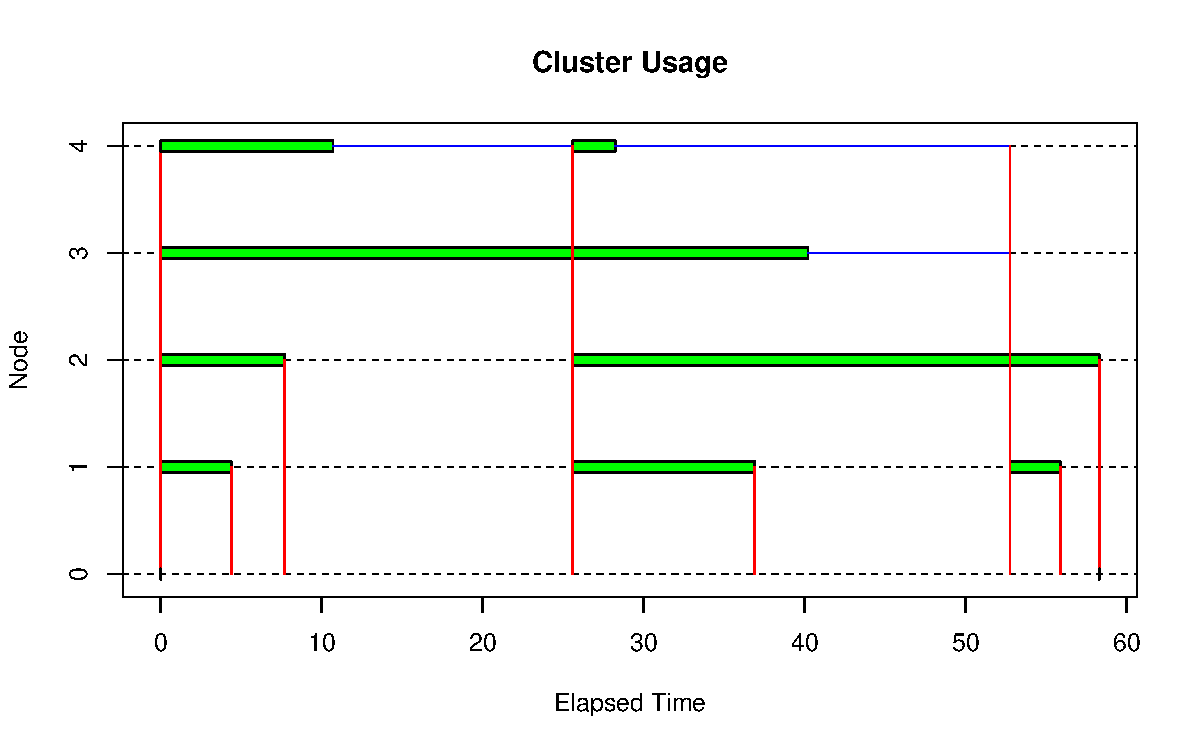
\includegraphics[width=.89\linewidth]{figure/unnamed-chunk-9-1} 

\end{knitrout}
\end{frame}

\begin{frame}[fragile]{Load Balancing}

So we waited for more than 50 seconds. 
A more efficient way would be pull the tasks to clusters when they are needed.
This technique is called {\color{blue} ``load balancing''}. Function \texttt{clusterApplyLB()} uses that technique.


\begin{knitrout}\scriptsize
\definecolor{shadecolor}{rgb}{1, 1, 1}\color{fgcolor}\begin{kframe}
\begin{alltt}
\hlkwd{set.seed}\hlstd{(}\hlnum{123}\hlstd{)}
\hlstd{sleeptime} \hlkwb{<-} \hlkwd{abs}\hlstd{(}\hlkwd{rnorm}\hlstd{(}\hlnum{10}\hlstd{,} \hlnum{10}\hlstd{,} \hlnum{10}\hlstd{))}
\hlstd{tm} \hlkwb{<-} \hlkwd{snow.time}\hlstd{(}\hlkwd{clusterApplyLB}\hlstd{(cl, sleeptime, Sys.sleep))}
\end{alltt}
\end{kframe}
\end{knitrout}
\end{frame}

\begin{frame}[fragile]{Load Balancing}
\begin{knitrout}\tiny
\definecolor{shadecolor}{rgb}{1, 1, 1}\color{fgcolor}
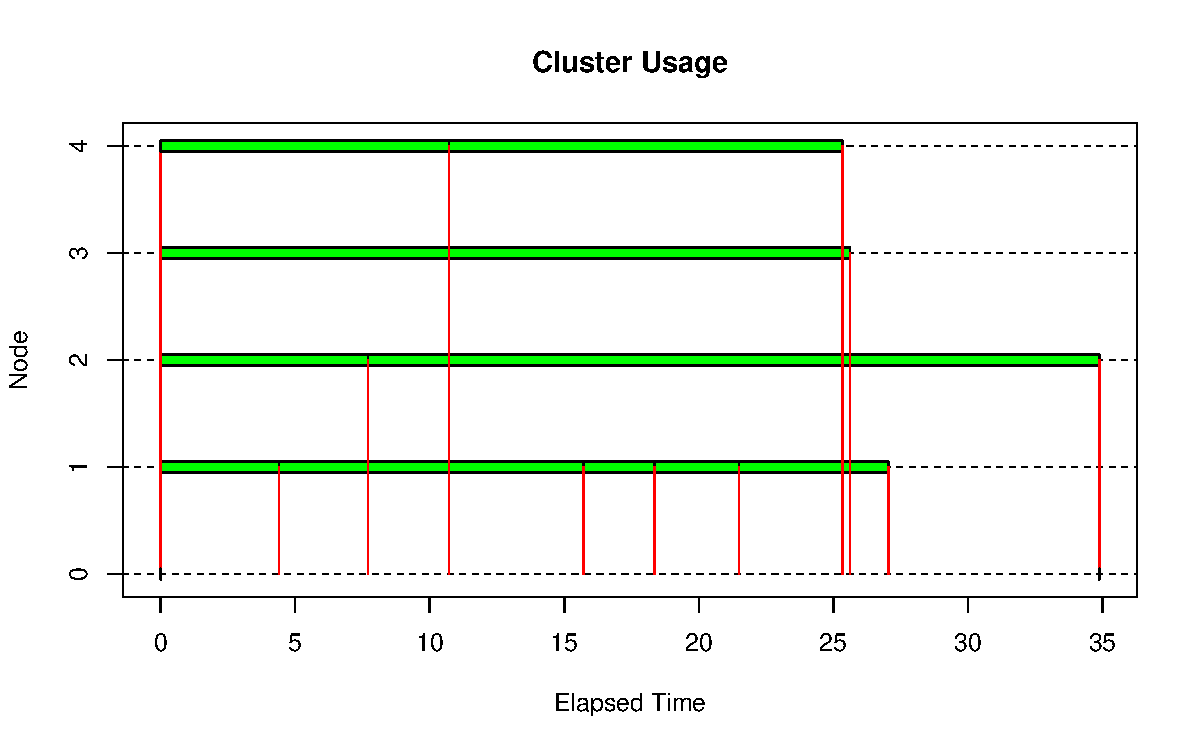
\includegraphics[width=.89\linewidth]{figure/unnamed-chunk-12-1} 

\end{knitrout}
\end{frame}

\begin{frame}{Load Balancing}
  So, here we waited for about 30 seconds. This is an improvement. The only wasted time was at the end. 
\end{frame}

\begin{frame}[fragile]{High-level API}
%   \begin{itemize}
%     \item parLapply(cl, x, fun, \ldots) --- parallel version of lapply()
%     \item parSapply(cl, X, FUN, \ldots, simplify = TRUE, USE.NAMES = TRUE) --- parallel version of sapply()
%     \item parApply(cl, X, MARGIN, FUN, \ldots) --- parallel version of apply()
%     \item parRapply(cl, x, fun, \ldots) --- row apply() for matrix
%     \item parCapply(cl, x, fun, \ldots) --- col apply() for matrix.
%   \end{itemize}
  
  \begin{table}[]
    \rowcolors{1}{gray!25}{white}
    \centering
    \begin{tabular}{ll}
      \texttt{parLapply(cl, x, fun, \ldots)} & Parallel version of lapply(). \\
      \begin{tabular}{@{}l@{}}
        \texttt{parSapply(cl, X, FUN, \ldots,} \\ 
        \quad \texttt{simplify = TRUE, USE.NAMES = TRUE)}
      \end{tabular} & 
      \begin{tabular}{@{}l@{}}
        Load Balancing version of \\ clusterApply(). 
      \end{tabular} \\
      \texttt{parApply(cl, X, MARGIN, FUN, \ldots)} & 
         Parallel version of apply(). \\
      \texttt{parRapply(cl, x, fun, \ldots)} & 
         \begin{tabular}{@{}l@{}}
           Row apply() for matrix.
         \end{tabular} \\
       \begin{tabular}{@{}l@{}}
          \texttt{parCapply(cl, x, fun, \ldots)}
        \end{tabular}
        & Column apply() for matrix.
    \end{tabular}
  \end{table}

  \bigskip
  
  The most useful is \texttt{parLapply()} function. It is different from \texttt{clusterApply()} because it splits the task into ``equal'' tasks.
\begin{knitrout}\scriptsize
\definecolor{shadecolor}{rgb}{1, 1, 1}\color{fgcolor}\begin{kframe}
\begin{alltt}
\hlstd{parLapply}
\end{alltt}
\begin{verbatim}
## function (cl, x, fun, ...) 
## docall(c, clusterApply(cl, splitList(x, length(cl)), lapply, 
##     fun, ...))
## <environment: namespace:snow>
\end{verbatim}
\end{kframe}
\end{knitrout}
where \texttt{splitList()} is an internal snow function. 
\end{frame}

\begin{frame}[fragile]{Example of comparison clusterApply() and parLapply()}
  \texttt{parLapply()} could be more efficient if you have more tasks than workers.
  Another situation --- you send large arguments to \texttt{parLapply()}.
  Let's take a look at the example.
\begin{knitrout}\scriptsize
\definecolor{shadecolor}{rgb}{1, 1, 1}\color{fgcolor}\begin{kframe}
\begin{alltt}
\hlstd{bigsleep} \hlkwb{<-} \hlkwa{function}\hlstd{(}\hlkwc{sleeptime}\hlstd{,} \hlkwc{mat}\hlstd{)} \hlkwd{Sys.sleep}\hlstd{(sleeptime)}
\hlstd{bigmatrix} \hlkwb{<-} \hlkwd{matrix}\hlstd{(}\hlnum{0}\hlstd{,} \hlnum{2000}\hlstd{,} \hlnum{2000}\hlstd{)}
\hlstd{sleeptime} \hlkwb{<-} \hlkwd{rep}\hlstd{(}\hlnum{1}\hlstd{,} \hlnum{100}\hlstd{)}
\end{alltt}
\end{kframe}
\end{knitrout}
  Firstly, let's try \texttt{clusterApply()}.
\end{frame}

\begin{frame}[fragile]{Example of comparison \texttt{clusterApply()} and \texttt{parLapply()}}
\begin{knitrout}\tiny
\definecolor{shadecolor}{rgb}{1, 1, 1}\color{fgcolor}
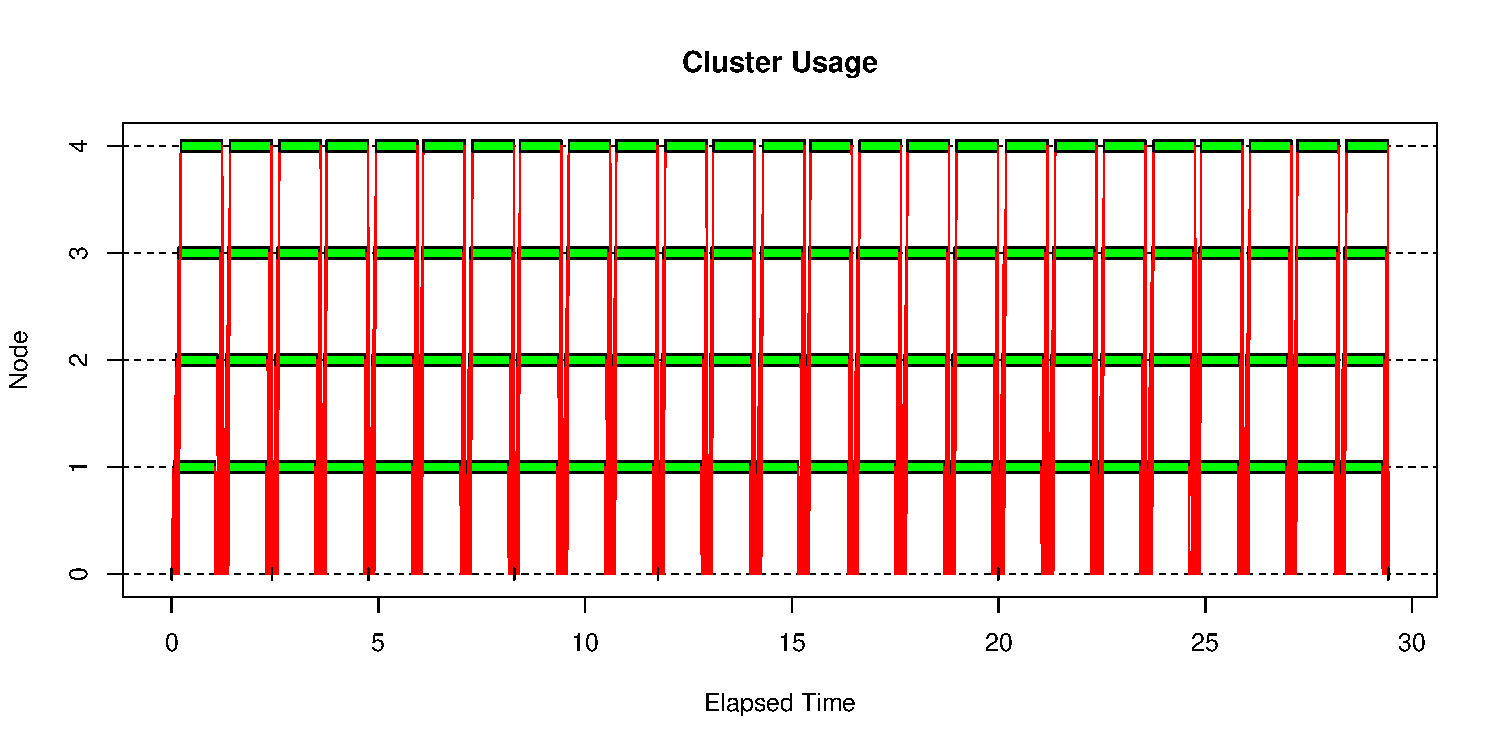
\includegraphics[width=.89\linewidth]{figure/unnamed-chunk-15-1} 

\end{knitrout}
\end{frame}

\begin{frame}[fragile]{Example of comparison \texttt{clusterApply()} and \texttt{parLapply()}}
  Definitely not highly efficient. Those gaps are due to I/O time.
  Ideally we should have 25 seconds... Let's give \texttt{parLapply()} a try.
\end{frame}

\begin{frame}[fragile]{Example of comparison \texttt{clusterApply()} and \texttt{parLapply()}}
\begin{knitrout}\tiny
\definecolor{shadecolor}{rgb}{1, 1, 1}\color{fgcolor}
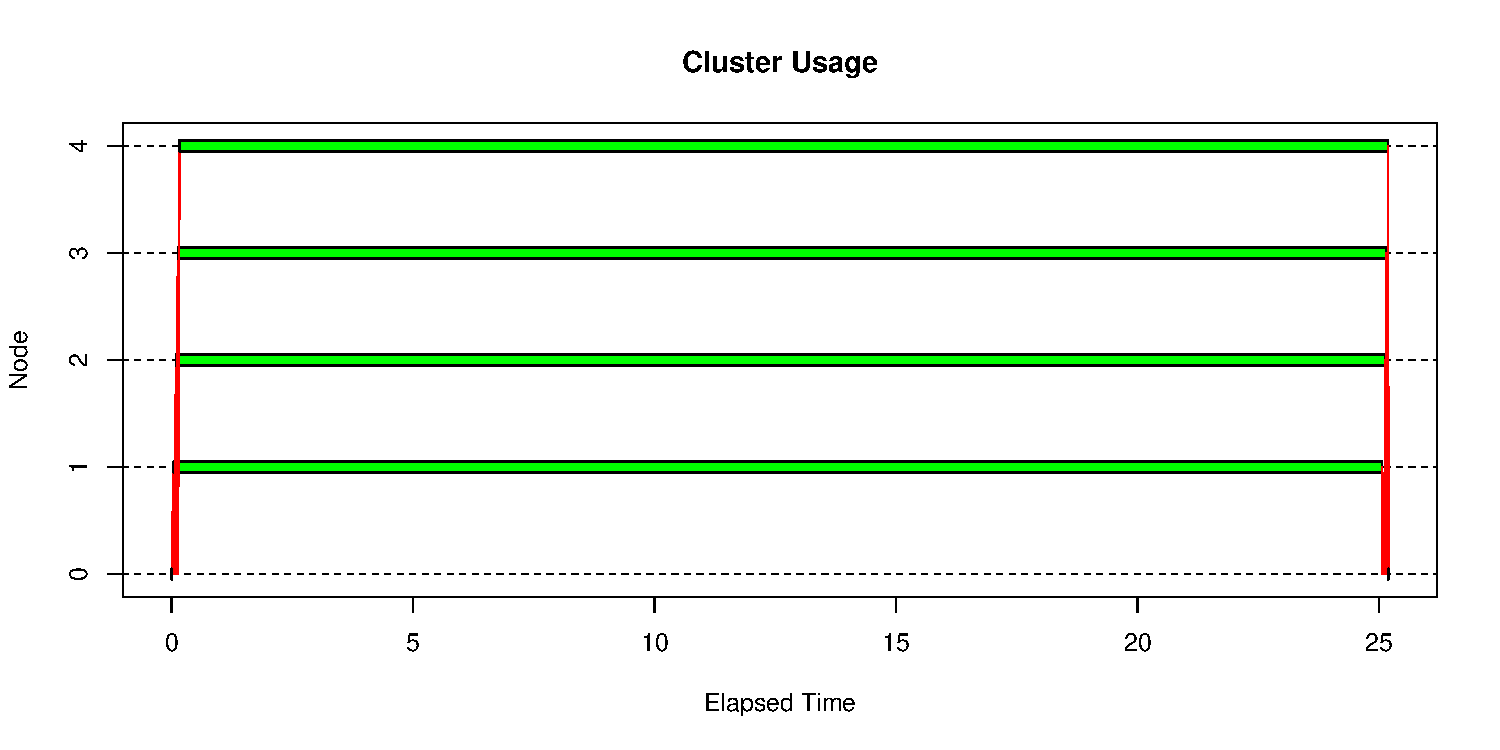
\includegraphics[width=.89\linewidth]{figure/unnamed-chunk-16-1} 

\end{knitrout}

\end{frame}

\begin{frame}[fragile]{Load Balancing parLapply?}
  \pause
  Short answer: no, there is no such a function in snow package. \\
  Good news: it is possible to write your own.
\end{frame}

\begin{frame}[fragile]{Random Number Generation}
  There are 2 basic steps.\\
  \begin{enumerate}
    \item Configure your cluster workers to use a generator.
\begin{knitrout}\scriptsize
\definecolor{shadecolor}{rgb}{1, 1, 1}\color{fgcolor}\begin{kframe}
\begin{alltt}
\hlkwd{library}\hlstd{(rlecuyer)}
\hlkwd{clusterSetupRNG}\hlstd{(cl,} \hlkwc{type} \hlstd{=} \hlstr{'RNGstream'}\hlstd{)}
\end{alltt}
\begin{verbatim}
## [1] "RNGstream"
\end{verbatim}
\end{kframe}
\end{knitrout}

    \item Be happy to generate your numbers.
\begin{knitrout}\scriptsize
\definecolor{shadecolor}{rgb}{1, 1, 1}\color{fgcolor}\begin{kframe}
\begin{alltt}
\hlkwd{unlist}\hlstd{(}\hlkwd{clusterCall}\hlstd{(cl, runif,} \hlnum{1}\hlstd{))}
\end{alltt}
\begin{verbatim}
## [1] 0.12701112 0.75958186 0.72850979 0.09570262
\end{verbatim}
\end{kframe}
\end{knitrout}

  \end{enumerate}
\end{frame}


\section{multicore}
\begin{frame}
  \frametitle{\texttt{Multicore}  \textit{[deprecated]} : quick look}
  If it is deprecated, why even think about it?
  \pause
  The reason is the package \texttt{parallel}. \textit{Wait a little bit...}\\
  \pause
  \begin{table}[]
    \centering
    \begin{tabular}{rl}
      \rowcolor{gray!25}
      \textit{General use case:} & \begin{tabular}{@{}l@{}} Main word is {\color{blue} fork} (thus no Windows support), \\ provides {\color{blue} implicit} parallelism. \end{tabular} \\
      \textit{Examples:} & \texttt{lapply()} runs for ages on your Intel Core i999. \\
      \rowcolor{gray!25}
      \textit{Solves:} & Single-threaded. \\
      \textit{Problems}: & 
        \begin{minipage}{4in}
          \vskip 4pt
          \begin{itemize}
            \item No Windows support.
            \item No internal RNG support.
            \item Runs only on one computer.
            \item Cannot be used with \textbf{R} \texttt{GUI}.
            \item No internal Load Balancing, however, it can be imitated.
          \end{itemize}
          \vskip 4pt
        \end{minipage} \\
      \pause
      {\color{blue} \textit{Warning:}} & \begin{tabular}{@{}l@{}} \color{blue} Jobs started by \texttt{multicore} share the same state (because of \texttt{fork)}. \end{tabular} 
    \end{tabular}
  \end{table}
\end{frame}

\begin{frame}
  \frametitle{\texttt{Multicore}  \textit{[deprecated]} : quick look}
  We will only consider \textit{high-level} API and let \textit{low-level} to be out-of-scope.
  \begin{table}[]
    \rowcolors{1}{gray!25}{white}
    \centering
    \begin{tabular}{ll}
      \texttt{mclapply()} & parallel version of \texttt{lapply()}. \\
      \begin{tabular}{@{}l@{}}
        \texttt{mcmapply()}
      \end{tabular} & 
      \begin{tabular}{@{}l@{}}
        parallel version of \texttt{mapply()}.
      \end{tabular} \\
      \texttt{pvec()} & 
         \begin{tabular}{@{}l@{}} Somewhat an high-level analog of \\ low-level \texttt{clusterSplit()} function. \end{tabular} \\
      \texttt{parallel()} and \texttt{collect()} & 
         \begin{tabular}{@{}l@{}}
           \texttt{parallel()} creates a new process with \texttt{fork()}, \\ evaluate expression in parallel and after that \\ the result is retrieved by the \texttt{collect()}.
         \end{tabular}
    \end{tabular}
  \end{table}
%   \begin{itemize}
%     \item \texttt{mclapply()} --- parallel version of \texttt{lapply()};
%     \item \texttt{mcmapply()} --- parallel version of \texttt{mapply()};
%     \item \texttt{pvec()} --- somewhat an high-level analog of low-level \texttt{clusterSplit()} function; 
%     \item \texttt{parallel()} and \texttt{collect()} --- \texttt{parallel()} creates a new process with \texttt{fork()}, evaluate expression in parallel and after that the result is retrieved by the \texttt{collect()}.
%  \end{itemize}
\end{frame}

\begin{frame}{\texttt{Multicore: mclapply}}
  \texttt{mclapply()} is a parallel \texttt{lapply()}.\\
  \bigskip
  Syntax is as follows:\\
  \texttt{mclapply(X, FUN, ..., 
         mc.preschedule = TRUE, mc.set.seed = TRUE,\\
         \quad mc.silent = FALSE, mc.cores = getOption("mc.cores"))} \\
  where \\
  \begin{enumerate}
    \item \texttt{mc.preschedule = TRUE} --- how jobs are created for \texttt{X}.
    \item \texttt{mc.set.seed = TRUE} --- do you need to randomly seed slaves, or fork it?
    \item \texttt{mc.silent = FALSE} --- hide info from `stdout' for all parallel forked processes. `stderr' is not affected.
    \item \texttt{mc.cores == getOption("mc.cores")} --- number of \textbf{workers} (not cores, actually) to start.
  \end{enumerate}
\end{frame}

\begin{frame}{\texttt{Multicore: mclapply, mc.preschedule}}
  \begin{columns}[T]
    \begin{column}{.48\textwidth}
      Meaning:
      \begin{itemize}
        \item TRUE: divide data in \texttt{mc.cores}-jobs beforehand and fork it to \texttt{mc.cores}-processes.
        \item FALSE: for each piece of data construct a new job (up to \texttt{mc.cores}).
      \end{itemize}
    \end{column}
    \pause
    \begin{column}{.48\textwidth}
      Rule of thumb: use
      \begin{itemize}
        \item TRUE: you don't need load balance (for instance, if there are lot's of values in the data).
        \item FALSE: the variance of job completion is very high (so, you need load balance).
      \end{itemize}    
    \end{column}
  \end{columns}
\end{frame}


\section{parallel}
\begin{frame}{\texttt{parallel}}

  \begin{table}[]
    \centering
    \begin{tabular}{rl}
      \rowcolor{gray!25}
      \textit{General use case:} & \begin{tabular}{@{}l@{}} Main word is {\color{blue} mainstream}, \\ almost a wrapper of \texttt{snow} and \texttt{multicore} packages. \end{tabular} \\
      \textit{Examples:} & Anything above. \\
      \rowcolor{gray!25}
      \textit{Solves:} & Single-threaded and (partially) memory-bound. \\
      \textit{Cool features}: & 
        \begin{minipage}{4in}
          \vskip 4pt
          \begin{itemize}
            \item Preinstalled into \textbf{R} since 2.14.0.
            \item Full RNG support with no dependency on \texttt{rlecuyer} package.
            \item Almost nothing to learn (if you are still awake).
            \item Can be easily used on any platform including Windows.
            \item Highly compatible with \texttt{snow} and \texttt{multicore}.
          \end{itemize}
          \vskip 4pt
        \end{minipage} \\
      \pause
      {\color{blue} \textit{Warning:}} & 
        \begin{tabular}{@{}l@{}} 
          \color{blue} On Windows you can't use more than one machine. \\ \color{blue} It also can be difficult to configure multiple Linux machines. 
        \end{tabular} 
    \end{tabular}
  \end{table}
\end{frame}

\begin{frame}[fragile]{\texttt{parallel : detectCores()}}
  How many cores?

\begin{knitrout}
\definecolor{shadecolor}{rgb}{1, 1, 1}\color{fgcolor}\begin{kframe}
\begin{alltt}
\hlkwd{library}\hlstd{(parallel)}
\hlstd{mc.cores} \hlkwb{<-} \hlkwd{detectCores}\hlstd{()}
\hlstd{mc.cores}
\end{alltt}
\begin{verbatim}
## [1] 8
\end{verbatim}
\end{kframe}
\end{knitrout}
  {\color{blue} \textit{Warning:} It is important to take into account that you maybe have hyper-threading.}
\end{frame}

\begin{frame}[fragile]{\texttt{Parallel} RNG}
  Unlike \texttt{snow} package no additional packages (like \texttt{rlecuyer}) are needed.
  \begin{columns}[T]
    \begin{column}{.48\textwidth}
        Fork (no Windows) way:

\begin{knitrout}\scriptsize
\definecolor{shadecolor}{rgb}{1, 1, 1}\color{fgcolor}\begin{kframe}
\begin{alltt}
\hlkwd{RNGkind}\hlstd{(}\hlstr{"L'Ecuyer-CMRG"}\hlstd{)}
\hlkwd{unlist}\hlstd{(}\hlkwd{mclapply}\hlstd{(}\hlkwd{rep}\hlstd{(}\hlnum{1}\hlstd{,}\hlnum{4}\hlstd{), runif))}
\end{alltt}
\begin{verbatim}
## [1] 0.3768615 0.3824588 0.3845725 0.9092709
\end{verbatim}
\end{kframe}
\end{knitrout}
    \end{column}
    \begin{column}{.48\textwidth}
        Cluster way:
\begin{knitrout}\scriptsize
\definecolor{shadecolor}{rgb}{1, 1, 1}\color{fgcolor}\begin{kframe}
\begin{alltt}
\hlkwd{detach}\hlstd{(}\hlstr{"package:snow"}\hlstd{,} \hlkwc{character.only}\hlstd{=}\hlnum{TRUE}\hlstd{)}
\hlkwd{library}\hlstd{(parallel)}
\hlkwd{RNGkind}\hlstd{(}\hlstr{"L'Ecuyer-CMRG"}\hlstd{)}
\hlstd{cl} \hlkwb{<-} \hlkwd{makeCluster}\hlstd{(}\hlnum{2}\hlstd{,} \hlkwc{type}\hlstd{=}\hlstr{"PSOCK"}\hlstd{)}
\hlkwd{unlist}\hlstd{(}\hlkwd{clusterCall}\hlstd{(cl,} \hlkwa{function}\hlstd{(}\hlkwc{x}\hlstd{)} \hlkwd{runif}\hlstd{(}\hlnum{2}\hlstd{)))}
\end{alltt}
\begin{verbatim}
## [1] 0.2540804 0.9748368 0.4398108 0.2789652
\end{verbatim}
\begin{alltt}
\hlkwd{stopCluster}\hlstd{(cl)}
\end{alltt}
\end{kframe}
\end{knitrout}

    \end{column}
  \end{columns}
\end{frame}
\begin{frame}[fragile]{\texttt{parallel} RNG: reproducible results}
    Basic way to get reproducible results would be \texttt{mc.reset.stream()} --- the parallel random number generator is reinitialized using the current seed
    on the master.

\begin{knitrout}\scriptsize
\definecolor{shadecolor}{rgb}{1, 1, 1}\color{fgcolor}\begin{kframe}
\begin{alltt}
\hlkwd{detach}\hlstd{(}\hlstr{"package:snow"}\hlstd{,} \hlkwc{character.only}\hlstd{=}\hlnum{TRUE}\hlstd{)}
\hlkwd{library}\hlstd{(parallel)}
\hlkwd{RNGkind}\hlstd{(}\hlstr{"L'Ecuyer-CMRG"}\hlstd{)}
\hlstd{cl} \hlkwb{<-} \hlkwd{makeCluster}\hlstd{(}\hlnum{2}\hlstd{,} \hlkwc{type}\hlstd{=}\hlstr{"PSOCK"}\hlstd{)}
\hlkwd{clusterSetRNGStream}\hlstd{(cl,} \hlnum{123}\hlstd{)}
\hlkwd{unlist}\hlstd{(}\hlkwd{clusterCall}\hlstd{(cl,} \hlkwa{function}\hlstd{(}\hlkwc{x}\hlstd{)} \hlkwd{runif}\hlstd{(}\hlnum{2}\hlstd{)))}
\end{alltt}
\begin{verbatim}
## [1] 0.1663742 0.3898457 0.3411064 0.9712727
\end{verbatim}
\begin{alltt}
\hlkwd{clusterSetRNGStream}\hlstd{(cl,} \hlnum{123}\hlstd{)}
\hlkwd{unlist}\hlstd{(}\hlkwd{clusterCall}\hlstd{(cl,} \hlkwa{function}\hlstd{(}\hlkwc{x}\hlstd{)} \hlkwd{runif}\hlstd{(}\hlnum{2}\hlstd{)))}
\end{alltt}
\begin{verbatim}
## [1] 0.1663742 0.3898457 0.3411064 0.9712727
\end{verbatim}
\begin{alltt}
\hlkwd{stopCluster}\hlstd{(cl)}
\end{alltt}
\end{kframe}
\end{knitrout}
\end{frame}

\begin{frame}{Differences from \texttt{multicore} and \texttt{snow}}
  Let's sum up the differences between modern \texttt{parallel} package and his predecessors.
  \begin{columns}[T]
    \begin{column}{.48\textwidth}
      \texttt{parallel} $>$ \texttt{multicore}
      \begin{itemize}
        \item Prefix \texttt{mc} in \texttt{mcfork()}, \texttt{mcexit()}, \texttt{mckill()}, \texttt{mcparallel()}, \texttt{mccollect()}, \texttt{mc.cores}.
        \item Different default value of \texttt{mc.cores} argument.
        \item New mc.reset.stream() function.
      \end{itemize}
    \end{column}
    \begin{column}{.48\textwidth}
      \texttt{parallel} $\neq$ \texttt{snow}
      \begin{itemize}
        \item New function \texttt{clusterSetRNGStream()} initializes parallel RNG.
        \item \texttt{snow.time()} function not included.
        \item \texttt{makeCluster()} supports additional types “FORK”.
      \end{itemize}
    \end{column}
  \end{columns}
  \bigskip
  Also useful \texttt{detectCores()} is added.
\end{frame}

\section{What else and references}

\begin{frame}{Out of scope}
  We covered 3 (2.5 really) packages: \texttt{snow}, \texttt{multicore}, \texttt{parallel}. What else?
  \begin{itemize}
    \item \textit{Revolution Analytics} \texttt{foreach} package for iteration over a set of values.
    \item MapReduce via Java Hadoop: \texttt{RHIPE} (negotiator between you with your MapReduce functions and Hadoop).
    \item \texttt{Segue} for Amazon Elastic MapReduce lovers. {\color{blue} Be aware of terminating clusters.}
    \item \texttt{doRedis}.
    \item \url{http://cloudNumbers.com}
    \item \textbf{R} and GPUs: \texttt{gputools} etc.
  \end{itemize}
\end{frame}

\begin{frame}{Literature}
  \begin{columns}[T]
    \begin{column}{.48\textwidth}
        Main reference: \\
        \includegraphics*[height=.8\textheight]{figure/Parallel_R.jpg} 
    \end{column}
    \begin{column}{.48\textwidth}
        \textbf{Useful links:}
        \begin{itemize}
          \item \href{http://adv-r.had.co.nz/}{Advanced \textbf{R}} by Hadley Wickham.
          \item \href{http://www.burns-stat.com/documents/books/the-r-inferno/}{The \textbf{R} Inferno} by Patrick Burns.
          \item \href{http://r-pkgs.had.co.nz/}{\textbf{R} Packages} by Hadley Wickham.
          \item \href{http://cran.r-project.org/doc/manuals/r-release/R-exts.html}{Writing \textbf{R} Extensions}.
          \item \href{http://www.bytemining.com/files/talks/larug/hpc2012/HPC_in_R_rev2012.pdf}{Los Angeles \textbf{R} Users’ Group: Parallelization in \textbf{R}, Revisited} by Ryan R. Rosario.
          \item \href{https://stat.ethz.ch/R-manual/R-devel/library/parallel/doc/parallel.pdf}{Package ‘parallel’ manual}.
        \end{itemize}
    \end{column}
  \end{columns}
\end{frame}

\end{document}
